\section{White-box Adversarial Examples}

% tikz illustration of L_p norms in a 2D coordinate system for p=0, 1, 2 and $\infty$.
% for each norm, we draw the 'circle' of points with distance 1 from the origin.
% for p=2, that is an actual circle, for p=1 it's a diamond, for p=$\infty$ it's a square and for p=0 it goes along the axes.
% each 'circle' should be labeled with the corresponding p as $\[ || x ||_p = 1 \]$.
% all illustrations should be in the same coordinate system, with the same scale.

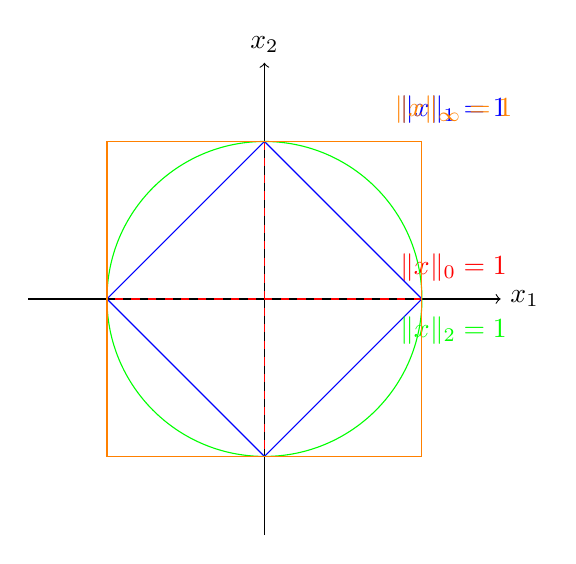
\begin{tikzpicture}[scale=2]

% Axes
\draw[->] (-1.5,0) -- (1.5,0) node[right] {$x_1$};
\draw[->] (0,-1.5) -- (0,1.5) node[above] {$x_2$};

% L_0 norm (along axes)
\draw[dashed,red] (1,0) -- (-1,0);
\draw[dashed,red] (0,1) -- (0,-1);
\node[red] at (1.2,0.2) {$\|x\|_0 = 1$};

% L_1 norm (diamond)
\draw[blue] (1,0) -- (0,1) -- (-1,0) -- (0,-1) -- cycle;
\node[blue] at (1.2,1.2) {$\|x\|_1 = 1$};

% L_2 norm (circle)
\draw[green] (0,0) circle (1);
\node[green] at (1.2,-0.2) {$\|x\|_2 = 1$};

% L_infinity norm (square)
\draw[orange] (1,1) -- (1,-1) -- (-1,-1) -- (-1,1) -- cycle;
\node[orange] at (1.2,1.2) {$\|x\|_\infty = 1$};

% Labels
\node at (1.4,0) [below] {};
\node at (0,1.4) [right] {};

\end{tikzpicture}
